\documentclass{article}
\usepackage[dutch]{babel}
\usepackage{hyperref}
\usepackage{graphicx}
\usepackage[bottom=2.5cm, right=2.5cm, left=2.5cm, top=2.5cm]{geometry}

\title{Eindvergadering ML sessie 5}
\author{Team $\exists$uler: \textit{Daan, Marie, Zeineb, Florian, Vincent, Jasper, Lasha, Younes}}
\date{Vrijdag \today}

\begin{document}
	
\maketitle

\section*{Reflectie}

Jasper en Younes hebben teksten gelezen i.v.m. onze extra toepassing, Support Vector Machines. Ze zijn daarnaast ook begonnen aan de uitleg en bijhorende illustraties.

 Lasha, Zeineb, Marie, Florian en Daan zijn begonnen aan de implementaties en zullen afwerken waar ze mee bezig waren. De status van het tabblad \textit{Implementatie} in de KanBan is te zien in figuur \ref{fig:kanban}.
 
 \section*{Simulatie 1}
 
 Vóór de aanvang van de sessie was simulatie 1 reeds in orde gebracht.
In deze simulatie hebben we een steekproef \((x_i, 10^{x_i} + \epsilon_i)\) van 20 punten met een standaardnormaal verdeeld residu en een uniform verdeelde regressor tussen 0 en 1. We stelden de steekproef grafisch voor, voegden de populatiefunctie toe, de regressielijn en de KNN-modellen voor \(K=1\), \(K=5\) en \(K=20\):

\begin{figure}[h!]
	\centering
	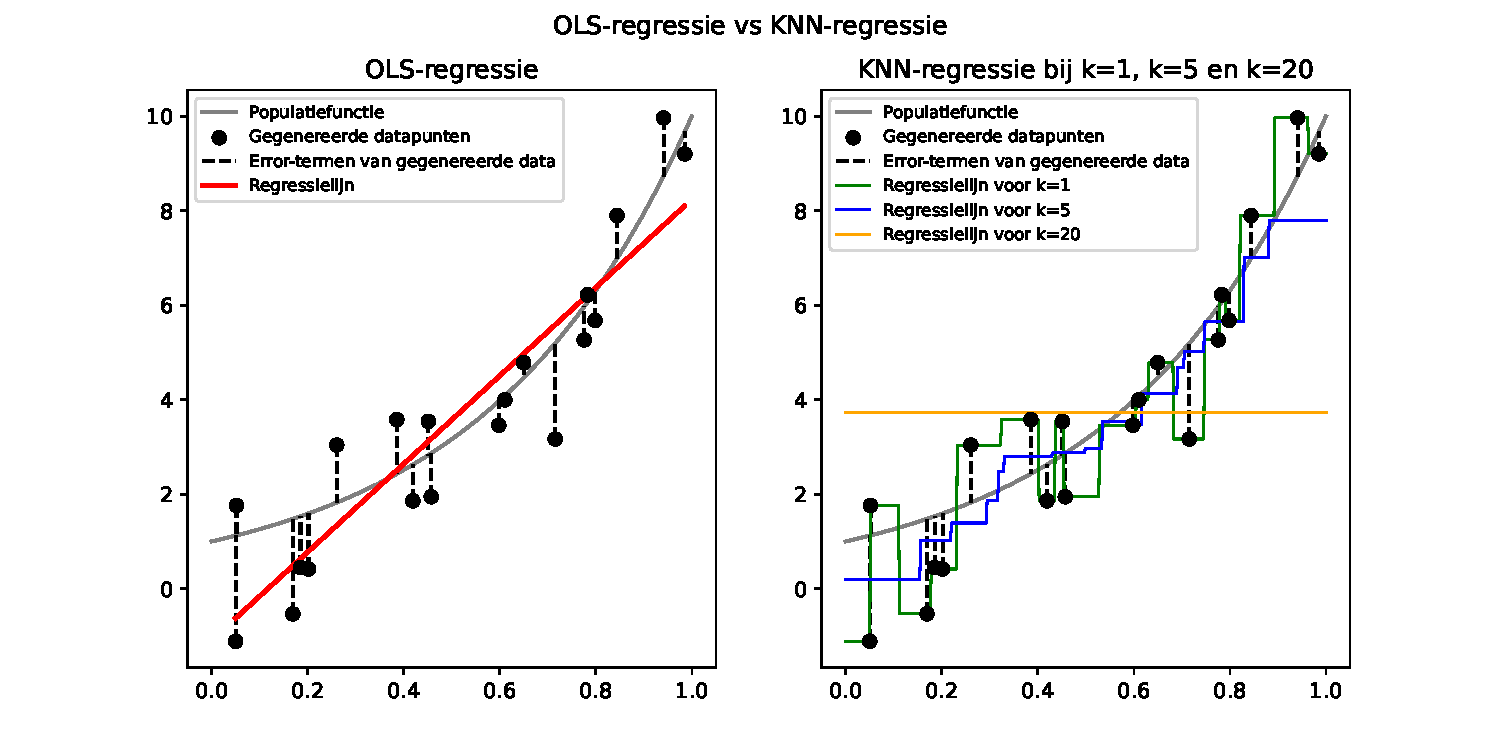
\includegraphics[width=0.8\textwidth]{simulatie1}
	\label{fig:simulatie1}
	\caption{OLS-regressie vergeleken met KNN-regressie voor verschillende waarden van \(K\).}
\end{figure}

De OLS-regressielijn is lineair, wat ervoor zorgt dat de populatiefunctie - die niet lineair is - niet super goed benaderd wordt.

Bij de (groene) KNN-regressielijn voor \(K=1\) is er duidelijk sprake van \textit{overfitting}: de regressielijn volgt elk datapunt perfect en wordt dus ook heel sterk beïnvloed door uitschieters. De (blauwe) regressielijn voor \(K=5\) heeft een lagere bias, aangezien deze regressielijn zich op de 5 dichtstbijzijnde buren baseert en dus veel minder gevoelig is voor uitschieters in de gegenereerde dataset. Wanneer \(K=20\), is de KNN-regressielijn een rechte waarvan de y-waarde gelijk is aan de gemiddelde y-waarde van alle datapunten, aangezien het aantal datapunten ook gelijk is aan 20. We besluiten dus dat de regressielijn voor \(K=5\) de beste schatter is.

\begin{figure}
	\centering
	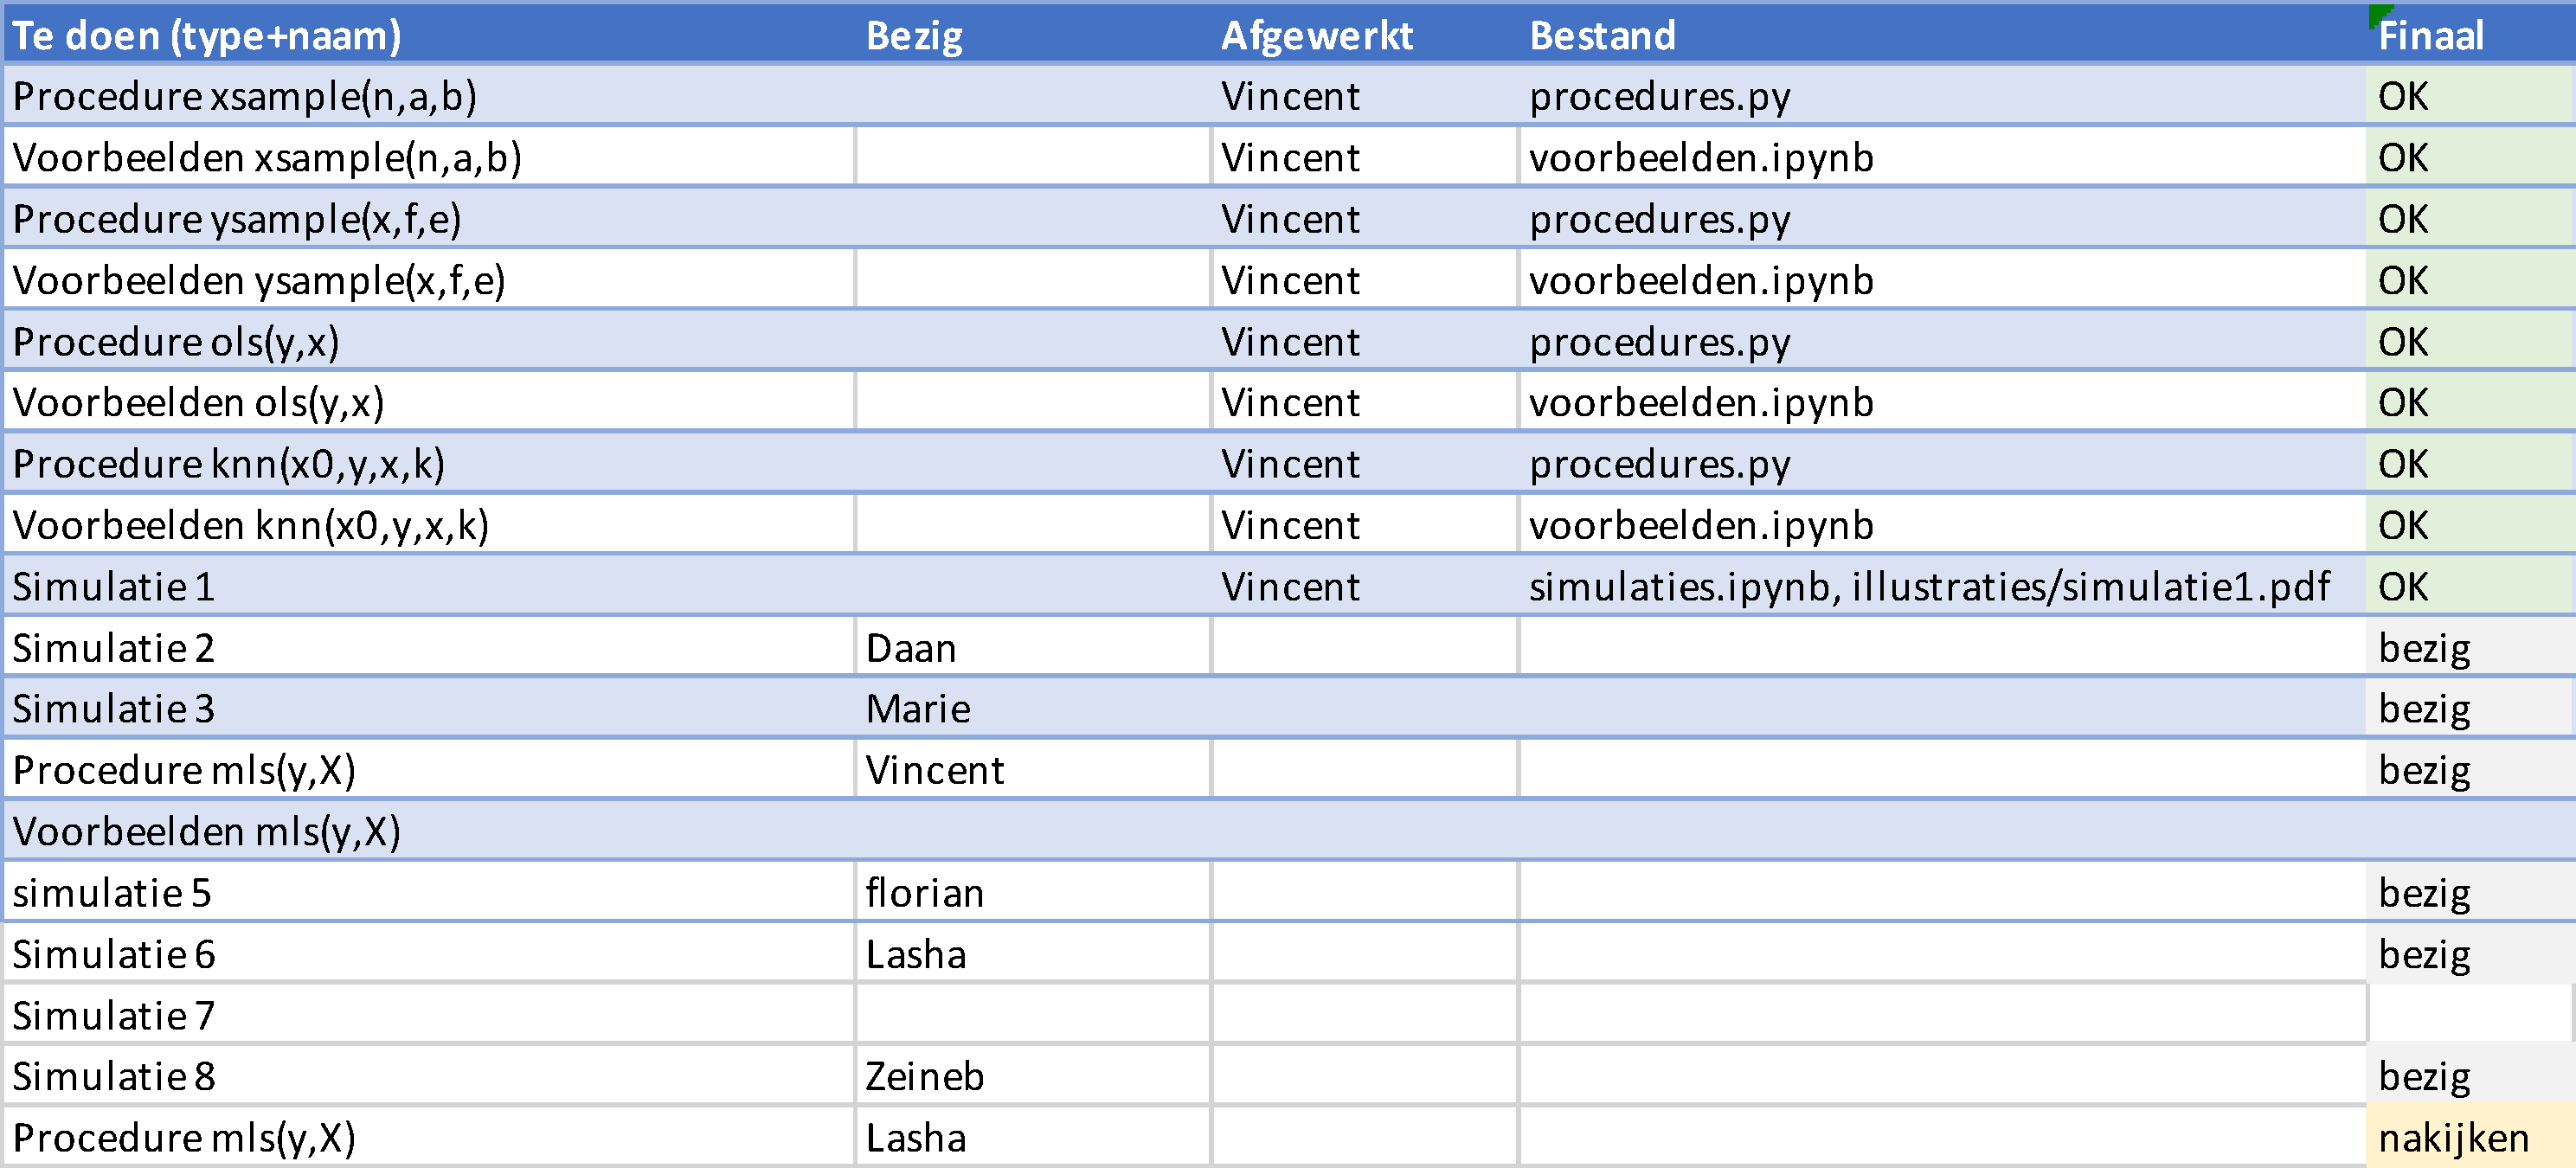
\includegraphics[width=0.9\textwidth]{kanban_einde}
	\caption{De status van het tabblad \textit{Implementatie} in de KanBan aan het einde van sessie 5}
	\label{fig:kanban}
\end{figure}

\section*{Vooruitblik}

De teamleden die startten met de implementatie van de basismethoden, zullen naar volgende week toe proberen afwerken waarmee ze bezig waren. Florian zal bovendien ook nog een oefening afwerken.

\end{document}